\documentclass[conference]{IEEEtran}
\IEEEoverridecommandlockouts

\usepackage{cite}
\usepackage{amsmath,amssymb,amsfonts}
\usepackage{graphicx}
\usepackage{textcomp}
\usepackage{xcolor}
\usepackage{booktabs}
\usepackage{url}
\usepackage{hyperref}

\def\BibTeX{{\rm B\kern-.05em{\sc i\kern-.025em b}\kern-.08em
    T\kern-.1667em\lower.7ex\hbox{E}\kern-.125emX}}

\begin{document}

\title{A Real-Time Data Collection System for Train Performance Analysis}

\author{
\IEEEauthorblockN{Arjun Sarje}
\IEEEauthorblockA{\textit{Department of Artificial Intelligence} \\
\textit{Samrat Ashok Technological Institute}\\
Vidisha, Madhya Pradesh, India \\
arjun27ai020@satiengg.in}
\and
\IEEEauthorblockN{Ashvin Sukaye}
\IEEEauthorblockA{\textit{Department of Artificial Intelligence} \\
\textit{Samrat Ashok Technological Institute}\\
Vidisha, Madhya Pradesh, India \\
ashvin27ai023@satiengg.in}
}


\maketitle

\begin{abstract}
Indian Railways is among the largest rail transportation systems globally, yet the ecosystem lacks an open, high-granularity, machine-learning-ready corpus for real-time delay analysis at station resolution. We present an automated, serverless data engineering pipeline that performs periodic polling of a live RailRadar REST API, orchestrated via GitHub Actions cron workflows, and persists normalized journey-state and station-event records in Supabase PostgreSQL. The system tracks end-to-end journey lifecycles for both single-day and multi-day services using a state-driven completion framework with failure-tolerant retry logic and idempotent storage constraints. Over an initial 1-month collection period (January 2026), with collection planned through April 2026, the pipeline monitors 10 representative trains (4 single-day, 6 multi-day) and captures approximately 15,000 station-level observations, including scheduled and observed arrival/departure timestamps, delay variables, and cumulative distance features. We formalize the collection methodology, schema design, and data-quality controls, and discuss sampling/operational biases inherent to API-mediated telemetry. The resulting open dataset establishes a reproducible benchmark for delay propagation modeling, ETA forecasting, timetable robustness analysis, and passenger information optimization in the Indian Railways context.
\end{abstract}

\begin{IEEEkeywords}
Indian Railways, railway delay analytics, real-time data pipeline, serverless architecture, GitHub Actions, cron scheduling, RESTful API ingestion, Supabase PostgreSQL, journey state tracking, delay propagation modeling, ETA prediction, transportation data engineering, reproducible dataset
\end{IEEEkeywords}

\section{Introduction}

Indian Railways operates one of the world's largest rail networks, serving over 8 billion passengers annually across approximately 68,000 km of track \cite{indian_railways_stats}. In such high-density, tightly coupled transportation systems, delay accumulation and propagation are not merely operational inconveniences; they are system-level phenomena that affect rolling-stock utilization, crew and platform scheduling, downstream connectivity, freight movement, and passenger reliability metrics. Consequently, robust delay modeling requires longitudinal, station-level, time-indexed observations that capture both intra-journey dynamics and inter-station propagation effects.

From a data systems perspective, the Indian Railways research ecosystem remains constrained by the absence of an openly accessible, continuously updated, and methodologically reproducible delay dataset. To address this gap, we design and deploy a cloud-native, serverless collection architecture that integrates scheduled workflow orchestration (GitHub Actions cron jobs), real-time REST API acquisition (RailRadar), and relational persistence (Supabase PostgreSQL) for lifecycle-aware train journey tracking. This design enables repeatable acquisition of structured operational telemetry suitable for statistical analysis and machine learning workflows.

\subsection{Problem Statement}

Although railway operators in Europe, Japan, and North America publish structured operational datasets that support reproducible performance analytics \cite{uk_rail_data, german_rail_data}, Indian Railways does not yet offer a public, high-granularity dataset with station-level and time-resolved delay observations suitable for real-time modeling and longitudinal analysis. Consequently, existing studies on Indian railway delays are typically constrained to low-fidelity or non-reproducible data sources, including:

\begin{itemize}
    \item Aggregated annual or periodic reports with coarse temporal granularity and limited station-level observability
    \item Manually collected survey datasets prone to sampling bias, observer inconsistency, and sparse temporal coverage
    \item Proprietary or institution-specific datasets that are inaccessible for independent validation and comparative benchmarking
    \item Anecdotal complaint records that lack standardized operational metadata (e.g., scheduled vs.\ actual event timestamps)
\end{itemize}

This data deficit materially limits the development and external validation of data-driven methods for delay prediction, timetable optimization, and passenger information systems. In particular, the absence of complete journey-lifecycle, station-wise delay traces impedes rigorous analysis of delay propagation dynamics, bottleneck localization, and route-level service reliability. Addressing this gap requires an open, continuously collected, and methodologically reproducible dataset generated through automated pipeline orchestration and state-aware journey tracking.

\subsection{Motivation and Contributions}

This work addresses the aforementioned gap by introducing:

\begin{enumerate}
    \item \textbf{Automated Data Collection System}: A stateless, scalable architecture for continuous real-time data acquisition from the RailRadar API
    \item \textbf{Public Dataset}: Station-wise delay records for 10 representative trains covering both single-day and multi-day journeys
    \item \textbf{Journey Lifecycle Tracking}: Complete documentation from journey initiation to completion, capturing temporal evolution of delays
    \item \textbf{Transparent Methodology}: Open-source implementation enabling reproducibility and extension by other researchers
\end{enumerate}

Our dataset, collected from January 1, 2026, comprises approximately 15,000 records spanning one month, with ongoing collection planned through April 2026. This resource enables empirical research in delay prediction, schedule reliability analysis, and transportation network optimization specific to Indian Railways.

\section{Related Work and Research Gaps}

\subsection{International Railway Delay Studies}

Extensive research exists on railway delay prediction and analysis in developed countries. European railways have been particularly well-studied due to open data initiatives. Oneto et al. \cite{oneto2018train} developed machine learning models for delay prediction using Deutsche Bahn data, achieving accuracy rates above 85\% for short-term forecasts. Similarly, UK railway performance datasets have enabled research on delay propagation \cite{flier2009delay} and timetable optimization \cite{goverde2010railway}.

Japanese railway systems, known for exceptional punctuality, have been analyzed for best practices in schedule adherence \cite{tomii2005train}. These studies benefit from comprehensive, publicly available datasets with minute-level granularity spanning multiple years.

\subsection{Indian Railway Research}

Research on Indian Railways faces significant data constraints. Existing studies fall into several categories:

\begin{itemize}
    \item \textbf{Survey-based studies}: Rely on passenger surveys or manual data collection at limited stations, introducing sampling bias and temporal gaps \cite{india_survey_example}
    \item \textbf{Simulation models}: Use theoretical models and assumed parameters due to lack of empirical data \cite{india_simulation_example}
    \item \textbf{Case studies}: Focus on specific routes or incidents without systematic data collection
    \item \textbf{Policy analysis}: Examine organizational factors without quantitative performance metrics
\end{itemize}

\subsection{Identified Gaps}

Our literature review reveals critical deficiencies in Indian railway delay research:

\begin{enumerate}
    \item \textbf{No Public Real-Time Datasets}: Unlike European and Japanese counterparts, no publicly accessible dataset captures real-time Indian railway performance
    \item \textbf{Limited Granularity}: Existing data lacks station-level detail necessary for bottleneck analysis
    \item \textbf{Incomplete Journey Coverage}: Previous studies do not track complete journey lifecycles from origin to destination
    \item \textbf{Multi-Day Journey Gap}: Long-distance trains spanning multiple days remain understudied
    \item \textbf{Reproducibility Issues}: Proprietary or manual data collection methods prevent independent verification
\end{enumerate}

Our work directly addresses these gaps by providing an open, automated, and continuously updated dataset with station-level granularity for both single-day and multi-day journeys.

\section{Methodology}

\subsection{System Architecture}

Our data collection system employs a serverless, cloud-based architecture designed for reliability and scalability (Fig. \ref{fig:architecture}). The system architecture consists of three primary components:

\begin{enumerate}
    \item \textbf{Automated Scheduler \& Executor}: GitHub Actions workflows with cron-based triggers execute Python polling scripts at configurable intervals (every 5 hours for single-day trains, every 12 hours for multi-day trains) on ephemeral Ubuntu runners
    \item \textbf{Data Source}: RailRadar API provides real-time train location and delay information via RESTful endpoints
    \item \textbf{Persistent Storage}: Supabase PostgreSQL database stores journey metadata and station-level records
\end{enumerate}

\begin{figure}[t]
\centering
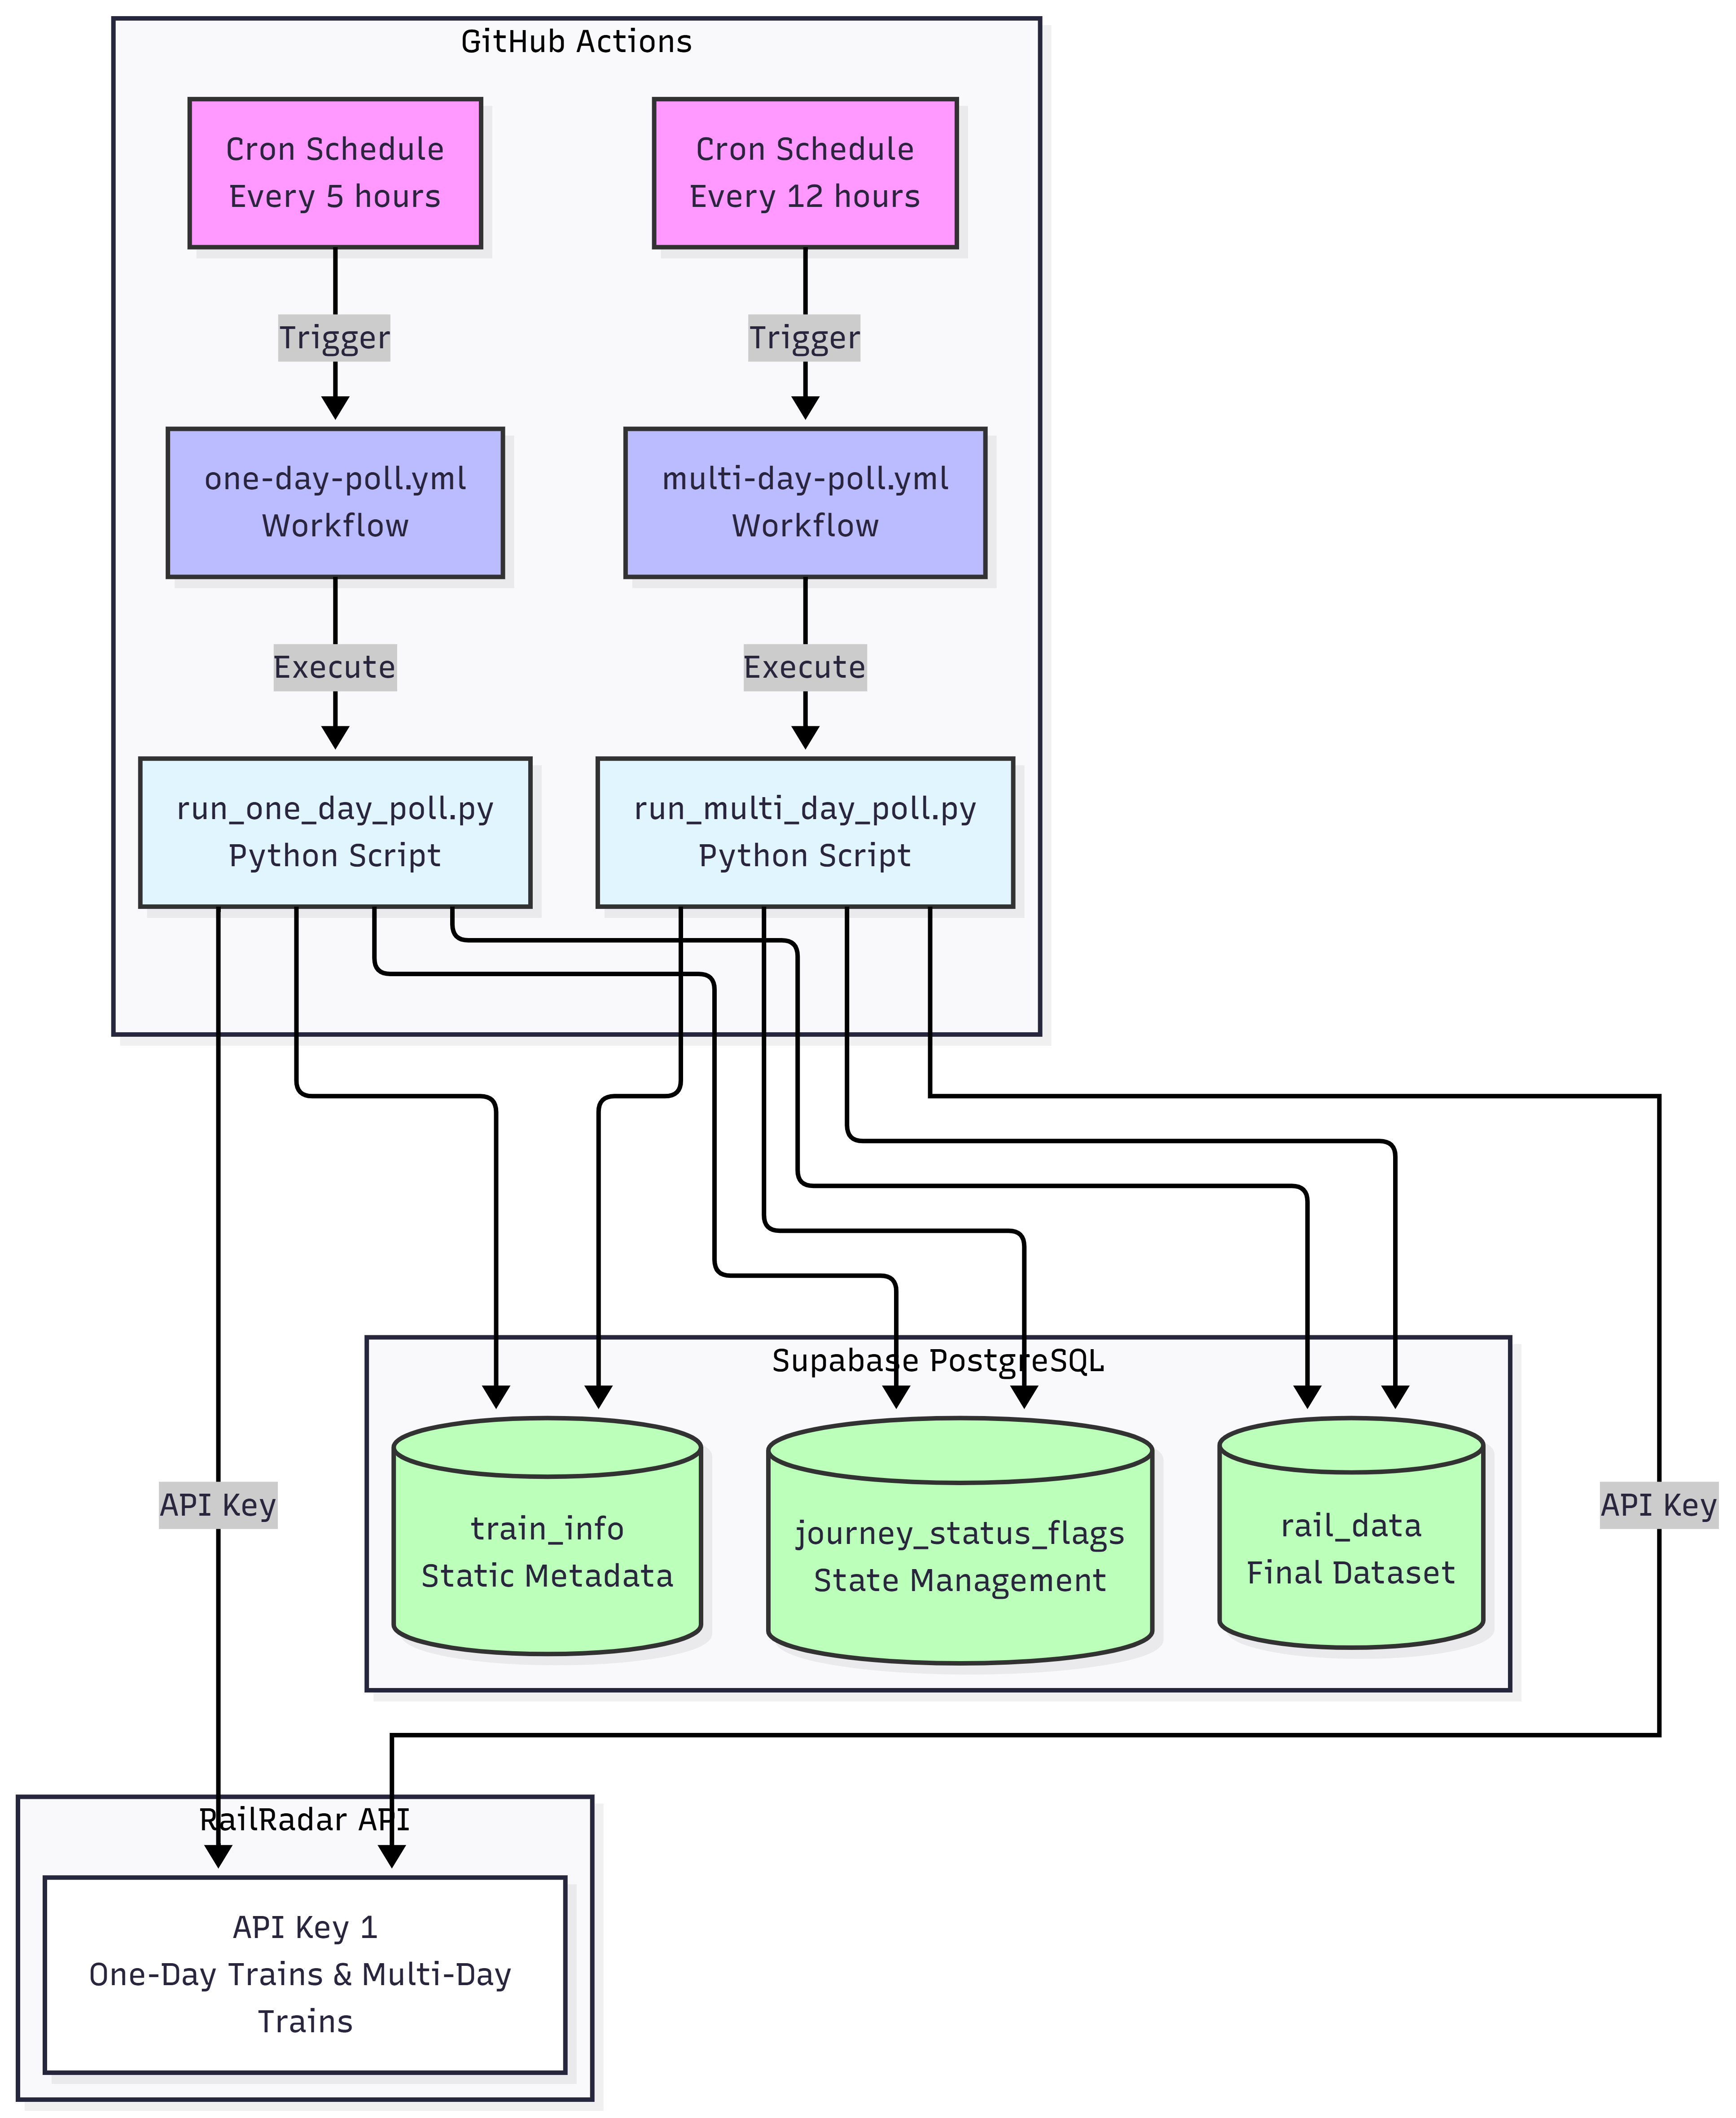
\includegraphics[width=\columnwidth]{system_architecture.png}
\caption{System architecture showing GitHub Actions schedulers triggering Python polling scripts that query RailRadar API and store data in Supabase PostgreSQL database with three interconnected tables.}
\label{fig:architecture}
\end{figure}

This serverless design eliminates the need for persistent web hosting infrastructure while ensuring data consistency through database-driven state management. GitHub Actions provides free computational resources for public repositories and reliable scheduled execution, making it ideal for periodic data collection tasks.

\subsection{RailRadar API Overview}

RailRadar is a comprehensive live train tracking platform for Indian Railways, providing real-time location data, delay information, and schedule details for over 13,000 trains across 10,000+ stations \cite{railradar_about}. The platform aggregates data through multiple sources including continuous web scraping of third-party railway information websites, Google Maps integration for train positioning validation, and manual database updates by their team. RailRadar operates independently of official government entities (NTES, Indian Railways), employing advanced error recovery and cross-verification systems to ensure data accuracy. Their RESTful API provides programmatic access to real-time train status, station information, and historical schedule data, enabling automated data collection systems like ours.

\subsection{Data Collection Workflow}

Our system implements a dual-phase polling strategy to efficiently track journey lifecycles:

\subsubsection{Phase 1: New Journey Detection}

For each monitored train, the system queries the RailRadar API daily to detect journey initiation. When a train's departure is confirmed (indicated by non-null live location data), a new journey record is created in the database with:

\begin{itemize}
    \item Train number and journey date (unique identifier)
    \item Completion status flags (initialized to incomplete)
    \item Tracking counter for API failure handling
\end{itemize}

\subsubsection{Phase 2: Ongoing Journey Tracking}

Active journeys are polled at regular intervals to monitor progress. For each incomplete journey, the system:

\begin{enumerate}
    \item Retrieves current train location from RailRadar API
    \item Compares current location with destination station
    \item If journey is incomplete, increments tracking counter
    \item If journey is complete, extracts full station-wise route data
    \item Stores scheduled times, actual times, delay values, and distances for all stations
\end{enumerate}

\subsection{Journey State Management}

The system implements a state machine to handle journey lifecycles (Fig. \ref{fig:state_machine}):

\begin{itemize}
    \item \textbf{Not Tracked}: Train not yet in system
    \item \textbf{In Progress}: Journey initiated, awaiting completion
    \item \textbf{Completed}: Train reached destination, all data recorded
    \item \textbf{Abandoned}: API failures exceeded threshold (6 consecutive failures), journey marked incomplete
\end{itemize}

\begin{figure}[t]
\centering
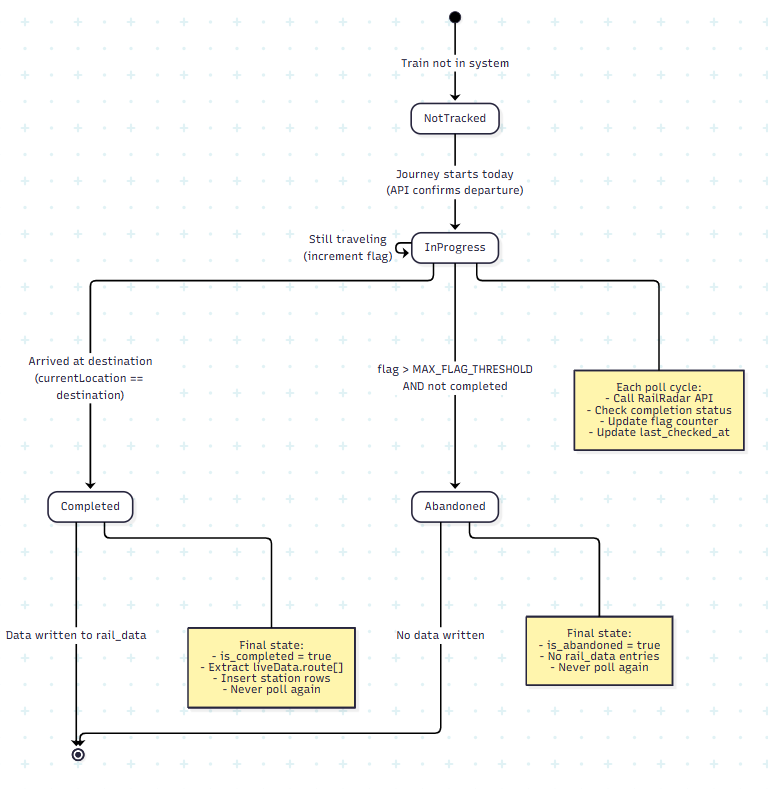
\includegraphics[width=\columnwidth]{journey_state_diagram.png}
\caption{Journey state machine showing transitions from Not Tracked through In Progress to either Completed (data written to rail\_data) or Abandoned (no data written) states.}
\label{fig:state_machine}
\end{figure}

This state-based approach ensures data integrity while gracefully handling API unavailability and network issues.

\subsection{Data Quality Measures}

To ensure dataset reliability, we implement several quality control mechanisms:

\begin{enumerate}
    \item \textbf{Idempotency}: Database constraints prevent duplicate records for the same train-journey-station combination
    \item \textbf{Timestamp Validation}: All times stored as Unix timestamps with timezone consistency (IST)
    \item \textbf{Failure Tolerance}: Transient API failures increment tracking counters rather than discarding journeys
    \item \textbf{Completion Verification}: Journey marked complete only when train's current location matches destination
\end{enumerate}

\subsection{Train Selection}

Our initial dataset covers 10 trains selected to represent diverse journey characteristics:

\begin{itemize}
    \item \textbf{4 Single-Day Trains}: Journeys completing within 24 hours, typically covering 300-800 km
    \item \textbf{6 Multi-Day Trains}: Long-distance journeys spanning 2-3 days, covering 1000-2500 km
\end{itemize}

This stratification enables comparative analysis between short-haul and long-haul delay patterns. Train selection prioritized daily service availability and route diversity across different geographic regions. Table \ref{tab:train_info} lists all 10 trains currently monitored in our system.

\begin{table*}[t]
\centering
\caption{Complete list of 10 trains monitored in the dataset}
\label{tab:train_info}
\small
\begin{tabular}{@{}clcccc@{}}
\toprule
\textbf{Train} & \textbf{Train Name} & \textbf{Journey} & \textbf{Destination} & \textbf{Duration} \\
\textbf{No.} & & \textbf{Type} & \textbf{Station} & \textbf{(hours)} \\
\midrule
61631 & Bhopal - Bina MEMU & one\_day & BINA & 3 \\
11605 & Bhopal - Bina MEMU Express & one\_day & BINA & 2 \\
11606 & Bina - Bhopal MEMU Express & one\_day & BPL & 2 \\
61632 & Bina - Bhopal MEMU & one\_day & BPL & 3 \\
12137 & Punjab Mail & multiple\_day & FZR & 33 \\
12138 & Punjab Mail & multiple\_day & CSMT & 33 \\
11077 & Jhelum Express  & multiple\_day & JAT & 40 \\
11078 & Jhelum Express & multiple\_day & PUNE & 40 \\
18237 & Chhattisgarh Express & multiple\_day & ASR & 43 \\
18238 & Chhattisgarh Express & multiple\_day & BSP & 42 \\
\bottomrule
\end{tabular}
\end{table*}

\section{Dataset Description}

\subsection{Data Schema}

The dataset comprises three interconnected tables:

\subsubsection{train\_info (Static Metadata)}
\begin{itemize}
    \item Train number, name, journey type
    \item Destination station code
    \item Expected journey duration
\end{itemize}

\subsubsection{journey\_status\_flags (Journey Tracking)}
\begin{itemize}
    \item Train number, journey date (composite key)
    \item Completion and abandonment flags
    \item API failure counter
    \item Last checked timestamp
\end{itemize}

\subsubsection{rail\_data (Core Dataset)}
\begin{itemize}
    \item Train number, journey date, station code (composite key)
    \item Scheduled arrival/departure timestamps (Unix format)
    \item Actual arrival/departure timestamps (Unix format)
    \item Delay in minutes (arrival and departure)
    \item Distance from origin in kilometers
\end{itemize}

\subsection{Dataset Statistics}

As of February 2026 (one month of collection), Table \ref{tab:dataset_stats} presents key statistics of the collected dataset.

\begin{table}[h]
\centering
\caption{Dataset Statistics (1 month)}
\label{tab:dataset_stats}
\begin{tabular}{@{}lc@{}}
\toprule
\textbf{Metric} & \textbf{Value} \\
\midrule
Total trains monitored & 10 \\
Single-day trains & 4 \\
Multi-day trains & 6 \\
Collection period & Jan 1-31, 2026 \\
Total station records & $\sim$15,000 \\
Completed journeys & $\sim$240 \\
Avg. stations per journey & $\sim$62 \\
Avg. duration (single-day) & 18 hours \\
Avg. duration (multi-day) & 42 hours \\
Collection frequency & 5h/12h \\
\bottomrule
\end{tabular}
\end{table}

\subsection{Journey Tracking Example}

Table \ref{tab:journey_flags} illustrates the journey\_status\_flags table, which tracks lifecycle state of each journey. The flag counter indicates API polling attempts before completion—Train 61631 completed immediately (flag=0), while Train 12137 required 3 polling cycles before reaching its destination after a 33-hour journey. All shown journeys completed successfully.

\begin{table}[h]
\centering
\caption{Sample journey tracking records}
\label{tab:journey_flags}
\small
\begin{tabular}{@{}ccccc@{}}
\toprule
\textbf{Train} & \textbf{Journey} & \textbf{Flag} & \textbf{Comp.} & \textbf{Aband.} \\
\textbf{No.} & \textbf{Date} & & & \\
\midrule
61631 & 2026-01-17 & 0 & true & false \\
11605 & 2026-01-17 & 0 & true & false \\
11606 & 2026-01-17 & 0 & true & false \\
61632 & 2026-01-17 & 2 & true & false \\
12137 & 2026-01-17 & 3 & true & false \\
\bottomrule
\end{tabular}
\end{table}

\subsection{Data Attributes}

Each station-level record contains:

\begin{itemize}
    \item \textbf{Temporal attributes}: Scheduled and actual arrival/departure times, enabling computation of dwell time, running time, and punctuality metrics
    \item \textbf{Delay measurements}: Separate delay values for arrival and departure, capturing station-specific delay dynamics
    \item \textbf{Spatial attributes}: Station code and cumulative distance from origin, enabling geographic analysis
    \item \textbf{Journey context}: Train number and journey date linking records to complete journey trajectory
\end{itemize}

\subsection{Data Example}

Table \ref{tab:data_example} presents sample records from the rail\_data table, illustrating typical station-level data structure. Train 61631's journey on January 17, 2026 shows progressively increasing delays at consecutive stations from 10-12 minutes at SMT to 18-20 minutes at GLG, demonstrating delay accumulation patterns common in Indian Railways operations.

\begin{table*}[t]
\centering
\caption{Sample station-level records showing delay progression}
\label{tab:data_example}
\small
\begin{tabular}{@{}ccccccccc@{}}
\toprule
\textbf{Train} & \textbf{Date} & \textbf{Station} & \textbf{Sched.} & \textbf{Sched.} & \textbf{Actual} & \textbf{Actual} & \textbf{Delay} & \textbf{Delay} \\
\textbf{No.} & & \textbf{Code} & \textbf{Arr.} & \textbf{Dep.} & \textbf{Arr.} & \textbf{Dep.} & \textbf{Arr.} & \textbf{Dep.} \\
& & & \textbf{(Unix)} & \textbf{(Unix)} & \textbf{(Unix)} & \textbf{(Unix)} & \textbf{(min)} & \textbf{(min)} \\
\midrule
61631 & 01-17 & SMT & 1768617720 & 1768617780 & 1768618314 & 1768618492 & 10 & 12 \\
61631 & 01-17 & SCI & 1768618140 & 1768618260 & 1768618886 & 1768619117 & 12 & 14 \\
61631 & 01-17 & BHS & 1768618800 & 1768618920 & 1768619665 & 1768619952 & 14 & 17 \\
61631 & 01-17 & SUMR & 1768619880 & 1768619940 & 1768620830 & 1768621132 & 16 & 20 \\
61631 & 01-17 & GLG & 1768620360 & 1768620480 & 1768621459 & 1768621704 & 18 & 20 \\
\bottomrule
\end{tabular}
\end{table*}

\subsection{Data Availability}

The dataset will be made publicly available under an open license upon completion of the 4-month collection period (January-April 2026). Interim data snapshots and collection code are available at \url{https://github.com/arz03/rail_data}.

\subsection{Known Limitations and Biases}

Transparency regarding dataset limitations is crucial for appropriate use:

\begin{enumerate}
    \item \textbf{Selection Bias}: Severely delayed journeys exceeding the abandonment threshold (6 consecutive API failures) are not recorded, potentially underrepresenting extreme delay scenarios
    \item \textbf{Sample Size}: 10 trains represent a small fraction of Indian Railways' 13,000+ trains, limiting generalizability
    \item \textbf{Geographic Bias}: Train selection may not uniformly cover all geographic regions and route types
    \item \textbf{Temporal Coverage}: One-month data may not capture seasonal variations or special event impacts
    \item \textbf{API Dependency}: Data quality depends on RailRadar API accuracy and availability
\end{enumerate}

These limitations should be considered when applying machine learning models trained on this dataset to operational scenarios.

\section{Applications and Future Scope}

\subsection{Immediate Applications}

This dataset enables several practical applications:

\subsubsection{Delay Prediction Models}
Station-level temporal data supports development of machine learning models for short-term delay forecasting, arrival time prediction at downstream stations, and delay propagation analysis across multi-station routes.

\subsubsection{Schedule Optimization}
Historical delay patterns can inform buffer time allocation in timetables, bottleneck identification at congested stations, and route-specific scheduling strategies.

\subsubsection{Passenger Information Systems}
Real-time and historical data integration can improve accurate arrival time displays at stations, journey planning with delay-aware recommendations, and passenger alert systems for significant delays.

\subsubsection{Station Congestion Analysis}
Dwell time and delay clustering analysis can identify stations with chronic congestion issues, peak congestion time windows, and infrastructure improvement priorities.

\subsection{Research Directions}

This dataset opens several research avenues including causal analysis of delay root causes through correlation with external factors, network effects on delay propagation, comparative studies benchmarking Indian Railways against international counterparts, and socioeconomic impact quantification.

\subsection{Dataset Extension Plans}

We plan to extend this work by increasing monitored trains to 50+ covering major routes, incorporating weather data and holiday calendars, continuing collection for 12+ months to capture seasonal variations, conducting ground-truth verification, and exploring multiple data sources for cross-validation.

\subsection{Community Contributions}

As an open dataset, we encourage community contributions for additional train coverage, feature engineering, baseline machine learning models, and visualization dashboards.

\section{Conclusion}

This paper presents the first publicly available, real-time dataset documenting Indian Railways train delays at station-level granularity. Our automated collection system addresses a critical gap in transportation research by providing empirical data previously inaccessible to the research community. The dataset's 15,000+ station records across 10 trains over one month—with ongoing expansion to four months—enables rigorous analysis of delay patterns, schedule reliability, and network performance.

Despite inherent limitations in sample size and selection bias, this dataset establishes a foundation for data-driven research in Indian railway operations. Applications in delay prediction, schedule optimization, and passenger information systems demonstrate immediate practical value. We anticipate this work will catalyze further research in railway analytics and inspire similar open data initiatives for other aspects of Indian Railways operations.

The complete dataset, collection system source code, and documentation will be publicly released under an open license, ensuring reproducibility and enabling community-driven extensions. By democratizing access to railway performance data, we hope to accelerate innovation in transportation analytics and contribute to improved service quality for millions of daily passengers.

\section*{Acknowledgments}

This research was conducted under the guidance of Dr. Rashi Kumari, Assistant Professor, Department of Artificial Intelligence, Samrat Ashok Technological Institute, Vidisha.

\begin{thebibliography}{00}
\bibitem{indian_railways_stats} Indian Railways, ``Indian Railways Annual Statistical Statements,'' Ministry of Railways, Government of India, 2024.

\bibitem{uk_rail_data} Network Rail, ``Network Rail Open Data Portal,'' \url{https://www.networkrail.co.uk/who-we-are/transparency-and-ethics/transparency/open-data-feeds/}, accessed January 2026.

\bibitem{german_rail_data} Deutsche Bahn, ``DB Open Data Portal,'' \url{https://data.deutschebahn.com/}, accessed January 2026.

\bibitem{oneto2018train} L. Oneto, E. Fumeo, G. Clerico, R. Canepa, F. Papa, C. Dambra, N. Mazzino, and D. Anguita, ``Train delay prediction systems: a big data analytics perspective,'' \textit{Big Data Research}, vol. 11, pp. 54--64, 2018.

\bibitem{flier2009delay} H. Flier, T. Graffagnino, and A. Nunkesser, ``Forecasting adverse weather impact on train delay in metropolitan areas,'' \textit{Transportation Research Part C: Emerging Technologies}, vol. 17, no. 3, pp. 270--286, 2009.

\bibitem{goverde2010railway} R. M. P. Goverde, ``A delay propagation algorithm for large-scale railway traffic networks,'' \textit{Transportation Research Part C: Emerging Technologies}, vol. 18, no. 3, pp. 269--287, 2010.

\bibitem{tomii2005train} N. Tomii, ``Train delay prediction model based on correlation analysis,'' in \textit{Proc. 1st Int. Seminar on Railway Operations Modelling and Analysis}, Delft, Netherlands, 2005.

\bibitem{india_survey_example} S. K. Mangla and P. Kumar, ``A study of passenger satisfaction and service quality in Indian Railways,'' \textit{Int. J. Logistics Systems and Management}, vol. 39, no. 3, pp. 331--356, 2021.

\bibitem{india_simulation_example} R. K. Agrawal and S. B. Dhamaniya, ``Simulation-based approach for analyzing train delays in Indian Railways,'' \textit{Transportation Research Procedia}, vol. 48, pp. 1726--1738, 2020.

\bibitem{railradar_about} RailRadar, ``About RailRadar - Live Train Tracking Platform,'' \url{https://railradar.in/about}, accessed January 2026.

\end{thebibliography}

\end{document}
